\documentclass[letterpaper]{article}

\usepackage{natbib,alifeconf}  %% The order is important


% *****************
%  Requirements:
% *****************
%
% - All pages sized consistently at 8.5 x 11 inches (US letter size).
% - PDF length <= 8 pages for full papers, <=2 pages for extended
%    abstracts (not including citations).
% - Abstract length <= 250 words.
% - No visible crop marks.
% - Images at no greater than 300 dpi, scaled at 100%.
% - Embedded open type fonts only.
% - All layers flattened.
% - No attachments.
% - All desired links active in the files.

% Note that the PDF file must not exceed 5 MB if it is to be indexed
% by Google Scholar. Additional information about Google Scholar
% can be found here:
% http://www.google.com/intl/en/scholar/inclusion.html.


% If your system does not generate letter format documents by default,
% you can use the following workflow:
% latex example
% bibtex example
% latex example ; latex example
% dvips -o example.ps -t letterSize example.dvi
% ps2pdf example.ps example.pdf


% For pdflatex users:
% The alifeconf style file loads the "graphicx" package, and
% this may lead some users of pdflatex to experience problems.
% These can be fixed by editing the alifeconf.sty file to specify:
% \usepackage[pdftex]{graphicx}
%   instead of
% \usepackage{graphicx}.
% The PDF output generated by pdflatex should match the required
% specifications and obviously the dvips and ps2pdf steps become
% unnecessary.


% Note:  Some laser printers have a serious problem printing TeX
% output. The use of ps type I fonts should avoid this problem.


\title{Brain Scaling In Evolved Braitenberg Vehicles}


%%do not add authors names, review process will be double blind 


\begin{document}
\maketitle

\begin{abstract}
% Abstract length should not exceed 250 word
  We provide an analysis of how neural dynamics
  change as a function of brain size in simulated agents. The agents 
  had neural network controllers optimized to solve the
  Braitenberg phototaxis task. We specifically consider the role of transient
  dynamics in orientation behavior. We find that the relationship between 
  transience of behavior and brain size is far from intuitive. We found that 
  although reliance on transience 
  We suggest that 
  this toy model may be useful as the reverse engineering approach to 
  cognition continues to grapple with foundational theoretical questions.
\end{abstract}

\section{Introduction}
The use of artificial neural network models to study cognition goes back to the very origins
of the artificial intelligence (cite). However, the average computational capabilities have
exploded since that time (cite). The ability to simulate larger and more complex networks 
has had a major impact on the field of neuroscience. The most recently popularized incarnation
of this research program, the Reverse Engineering approach, has emphasized the importance of 
large scale models in being able to connect theory to experimental data (cite).\\
One limitation of this approach is the trade-off between tractability and model complexity.
As models have more moving parts the harder it becomes to characterize and predict the 
relationships between those parts.\\
In much previous work such as in the evolutionary robotics literature (cite), 
toy models were used to gain theoretical insight. These models were then used to inform the development
of experimental models in less complex organisms (cite). Although even in the simplest nervous systems
we know of the number of components still seems intractable (cite).
Bridging the gap between simpler models with a
countable number of conponents and contemporary models of the Ventral visual stream for example, seems
like a daunting and potentially sysiphusian task.\\
However, sudge a bridge is necessary to build if we are to begin to unravel one of the greatest scientific
mysteries that still remains: our own minds. Toy models have given us important insights into which components
are important to driving behavior in cognitive systems, such as the importance of brain, body, environment
interactions in shaping cognition (cite). Many of these insights are still on their way to being incorporated
into the canon of the reverse engineering approach.\\
In this study we present an example of how future work may be pursued to connect these varied and important 
bodies of literature. We consider the effects of scaling in brain size to get a better understanding of
how model complexity may affect our understanding of systems of interest. We show that model complexity is
not simply a function of the brain size but also deeply depends on the task for which the system is optimized
for.

\section{Methods}
The goal of this paper is to study the effect of network size 
on neural dynamics. To do this we evolved neural network controllers
of different sizes to accomplish the same task with the same bodies.
This section describes the tasks, the neural network model, 
the evolutionary optimization algorithm and finally
the analysis methodologies used in this work.

\subsection{The Task}
In all cases the parameters for a neural network were evolved to 
solve a Braitenberg tropotaxis task. The task consisted of 8 different 
initial conditions. In each case the agent was initially placed in the 
center of a circle, with radius $r=5$, which is spanned by evenly spaced stimuli. Each
stimulus was present for one trial. An agent's fitness was a function
of their proximity to the each stimulus weighted by the time spent during the
trial. Agents with maximum fitness were thus those that could arrive at
the stimulus quickly and stay near it as long as possible. 
\begin{eqnarray}
  f(agent) = 1 - \frac{\sum^8_{i=1}\sum^T_{t=1}d(agent,stimuli_i)\cdot r}{T}
\end{eqnarray}
For ease of evaluation the equation above is clipped to be between [0,1].
Each trial lasted
for a duration of $T=50$ time units. The agents maximum velocity was constrained to
a single distance unit per time unit.
The agents have two sensors and two motors. The two sensors each recieve the inverse
distance to the stimulus as input.
The sum of the motor outputs determines the velocity of the agent. The difference
between the motor outputs determine the agents angular velocity. The velocities
were integrated during stimulation with Euler integration using a step size of 0.01

\subsection{Neural Network}
For the brain of the agent we use continious-time
recurrent neural netowrks (CTRNNs) with the following 
state equation (cite):
\begin{eqnarray} 
  \tau_i \dot(y)_i = -y_i + \sum_{j=i}^N w_{ji}\sigma(y_j+\theta_j)+s_i I_i
\end{eqnarray} 
where $y$ is the state of each node in the network. $\tau$ is time constant
for each node (in this case all $\tau$ are set to 1). $w_{ji}$ is the connection 
strength from node $j$ to node $i$.
$\theta$ is a bias term unique to each node. The function $\sigma = 1/(1+e^{-x})$.
$I_i$ is the inputs coming to sensory neuron $i$ weighted by sensory weight $s_i$.\\
The brain networks are fully connected. The weights are all bilaterally 
symmetric. Sensory input goes to two neurons in the network. Motor output is read
out by a linear readout of the entire network.
During simulation the network was simulated using Euler integration with a time-step
of 0.01. This is done in parallel with environmental simulation. We use networks of
sizes 2, 4, 8, 16, and 32.

\subsection{Evolutionary Algorithm}
The parameters of the neural circuits (all terms above) are evolved using a version
of the microbial genetic algorithm (cite). The parameters are encoded as a vector of real
numbers between [0,1]. At each step two individuals are selected. Their fitness is compared
the winner than transfers a random portion of their genes to the loser. The loser then mutates
their genome. The mutation is implemented as a random shift on each gene in the genome drawn
from a normal distribution with a mean of 0 and a variance inversely proportional to the number
of genes. \\
The population was initialized with 50 individuals. Evolution was preformed over the course of 
100 generations. We define one generation as 50 tournaments of 2 randomly selected individuals. 
Geography is induced where competing agents can only be selected from their 4 nearest neighbors 
along a 1D ring (cite).\\
The genome contains all parameters described above as well as the linear readout for the motor
output. Before being mapped back to parameters each gene in the genome is multiplied by its 
corresponding weight range. Biases, sensory and neural weights are constraned to a range of [-16,16].
Motor weights were constrained to [-1,1] however motor ouput was also normalized in the body duiring 
simulation to keep constant maximum speed regardless of brain size.

\section{Results}
\subsection{Successful Agents}
In all cases we were able to find agents which were successful at the tropotaxis
task. The agents used a large range of behaviorial dynamics

\subsection{Experiment 2}
\subsection{Experiment 3}

\section{Conclusion}


\section{Exponents and Power Laws}

\hyphenation{ap-proximated}

In this particular system avalanche size can be approximated
by the size $s$ of the genotype that gave rise to it,
Eq.~(\ref{size}).  We shall measure the distribution of these sizes
$P(s)$ in the Artificial Life system Avida, which implements a
population of self-replicating computer programs written in a simple
machine language-like instruction set of ${\cal D}=24$ instructions,
with programs of varying sequence length. In the course of
self-replication, these programs produce mutant off-spring because the
{\tt copy} instruction they use is flawed at a rate $R$ errors per
instruction copied, and adapt to an environment in which the
performance of {\em logical} computations on externally provided
numbers is akin to the catalysis of chemical reactions \citep{OBA}. In
this {\em artificial chemistry} therefore, successful computations
accelerate the metabolism (i.e., the CPU) of those strings that carry
the {\em gene} (code) necessary to perform the trick, and any program
discovering a new trick is the seed of another avalanche.

Avida is not a stirred-reactor environment (although one can be
simulated). Rather, the programs live on a two-dimensional grid, each
program occupying one site. The size of the grid is finite, and chosen
in these experiments to be small enough that avalanches are generally
over before a new one starts. As is well-known, this is the condition
{\em sine qua non} for the observation of SOC behavior, a separation
of time scales which implies that the system is driven at
infinitesimal rates.

Let $\tau$ denote the average duration of an avalanche. Then, a
separation of time scales occurs if the average time between the
production of new seeds of avalanches is much larger than $\tau$. New
seeds, in turn, are produced with a frequency $\langle\epsilon\rangle
P$, where $\langle\epsilon\rangle$ is again the average replication
rate, and $P$ is the mutation probability (per replication period) for
an average sequence of length $\ell$,
\begin{eqnarray}
P=1-(1-R)^\ell\;.
\end{eqnarray}
For small enough $R$ and not too large $\ell$ (so that the product
$R\ell$ is smaller than unity) we can approximate
$P\approx R\ell$, and infinitesimal driving occurs in the limit
\begin{eqnarray}
\langle \epsilon\rangle R\ell \ll\frac1\tau\;.\label{cond}
\end{eqnarray}
Furthermore
\begin{eqnarray}
\tau\sim\frac{L}v
\end{eqnarray}
with $L$ the diameter of the system and $v$ a typical Fisher velocity.
The fastest waves are those for which the latent heat is of the order
of the new fitness, i.e., $\Delta\epsilon\sim\epsilon$, in which case
$v\approx \epsilon$ \citep[because $D\sim\epsilon$ in
Eq.~(\ref{eq4}),][]{CHU}, and a separation of time scales is assured
whenever
\begin{eqnarray}
\frac1{R\ell}\gg {L}\;,
\end{eqnarray}
that is, in the limit of vanishing mutation rate or small population
sizes. For the $L=60$ system used here, this condition is obeyed (for
the fastest waves) only for the smallest mutation rate tested and
sequence lengths of the order of the ancestor.


\begin{figure}[t]
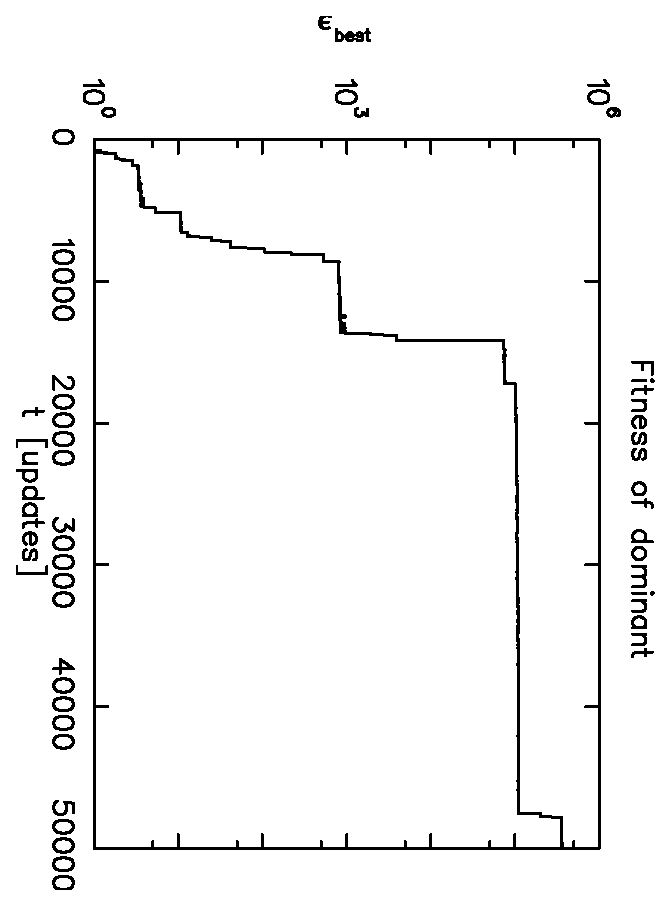
\includegraphics[width=2.3in, angle=90]{fig2.eps}
\caption{Fitness of the dominant genotype in the population, $\epsilon_{\rm best}$ as a function of time (in updates).}
\label{fig2}
\end{figure}


In the following, we keep the population size constant (a $60\times60$
grid) and vary the mutation rate. From the previous arguments, we
expect true scale-free dynamics only to appear in the limit of small
mutation rates.  As in this limit avalanches occur less and less
frequently, this is also the limit where data are increasingly
difficult to obtain, and other finite size effects can come into play.
We shall try to isolate the scale-free regime by fitting the
distribution to a power law
\begin{eqnarray}
P(s)\sim s^{-D(R)}\label{power}
\end{eqnarray}
and monitor the behavior of $D$ from low to high mutation rates.

In Fig.~\ref{fig2}, we display a typical history of $\epsilon_{\rm
best}$, i.e., the fitness of the dominant genotype.\footnote{As the
replication rate $\epsilon$ is exponential in the bonus obtained for a
successful computation, $\epsilon_{\rm best}$ increases exponentially
with time.}  Note the ``staircase'' structure of the curve reflecting
the ``punctuated'' dynamics, where each step reflects a new avalanche
and concurrently an extinction event. Staircases very much like these
are also observed in adapting populations of {\it E. Coli}
\citep{LT94}.

As touched upon earlier, the Avida world represents an environment
replete with information, which we encode by providing bonuses for
performing logical computations on externally provided (random)
numbers. The computations rewarded usually involve two inputs $A$ and
$B$, are finite in number and listed in Table~1. At the end of a
typical run (such as Fig.~\ref{fig2}) the population of programs is
usually proficient in almost all tasks for which bonuses are given
out, and the genome length has grown to several multiples of the
initial size to accommodate the acquired information.

\begin{table}[h]
\center{
\begin{tabular}{|c|c|c|c|}\hline
Name & Result & Bonus $b_i$ & Difficulty\\ \hline\hline
Echo & I/O   & 1 & --\\
Not  & $\neg A$ & 2 & 1 \\
Nand & $\neg(A\wedge B)$ & 2 & 1 \\
Not Or & $\neg A \vee B$ & 3 & 2 \\
And  &  $ A \wedge B $   & 3 & 2 \\
Or   &  $ A \vee B $     & 4 & 3 \\
And Not & $A\wedge\neg B$& 4 & 3 \\
Nor  & $\neg(A\vee B)$   & 5 & 4 \\
Xor  & $ A\ {\rm xor}\ B$ &   6 & 4 \\
Equals &$\neg(A\ {\rm xor}\ B)$&6& 4 \\ \hline
\end{tabular}
}
\vskip 0.25cm
\caption{Logical calculations on random inputs $A$ and $B$ rewarded,
bonuses, and difficulty (in minimum number of {\tt nand} instructions
required). Bonuses $b_i$ increase the speed of a CPU by a factor
$\nu_i=1+2^{b_i-3}$.}
\end{table}

Because the amount of information stored in the landscape is finite,
adaptation, and the associated avalanches, must stop when the
population has exhausted the landscape.  However, we shall see that
even a `flat' landscape (on which evolution is essentially neutral
after the sequence has optimized its replicative strategy) gives rise
to a power law of genotype sizes, as long as the programs do not
harbor an excessive amount of ``junk'' instructions.  A typical
abundance distribution (for the run depicted in Fig.~\ref{fig2}) is
shown in Fig.~\ref{fig3}.


\begin{figure}[ht]
\begin{center}
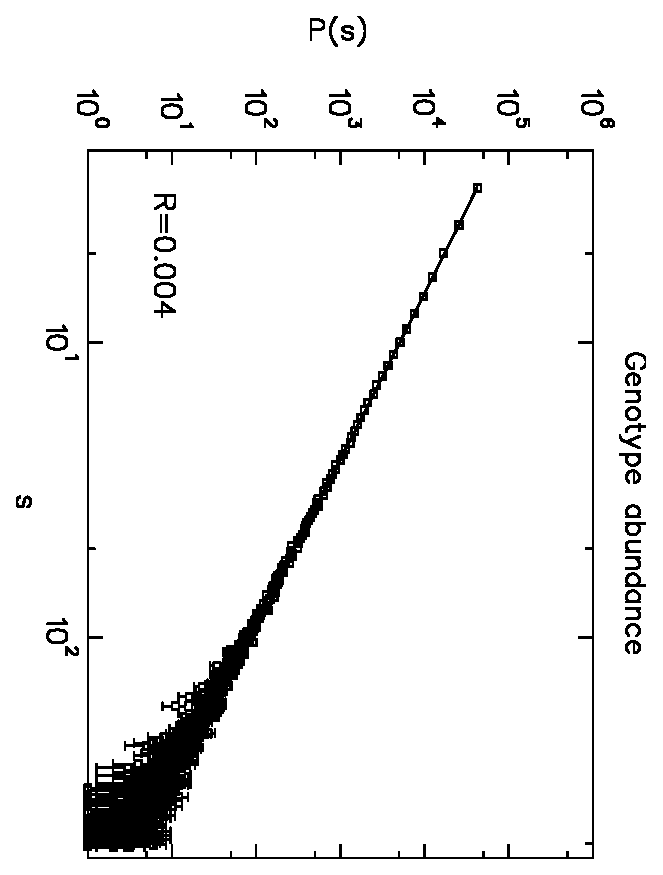
\includegraphics[width=2.25in, angle=90]{fig3.eps}
\caption{Distribution of genotypes sizes $P(s)$ fitted to a power law
  (solid line) at mutation rate $R=0.004$.}
\label{fig3}
\end{center}
\end{figure}


As mentioned earlier, we can also turn {\em off} all bonuses listed in
Tab.~1, in which case fitness is related to replicative abilities
only. Still, avalanches occur (within the first 50,000 updates
monitored) due to minute improvements in fitness, but the length of
the genomes typically stays in the range of the ancestor, a program of
length 31 instructions. We expect a change of dynamics once the
``true'' maximum of the local fitness landscape is reached, however,
we did not reach this regime in the experiments presented here. The
distribution of genotype sizes for the flat landscape is depicted in
Fig.~\ref{fig4}.


\begin{figure}[!tbp]
\begin{center}
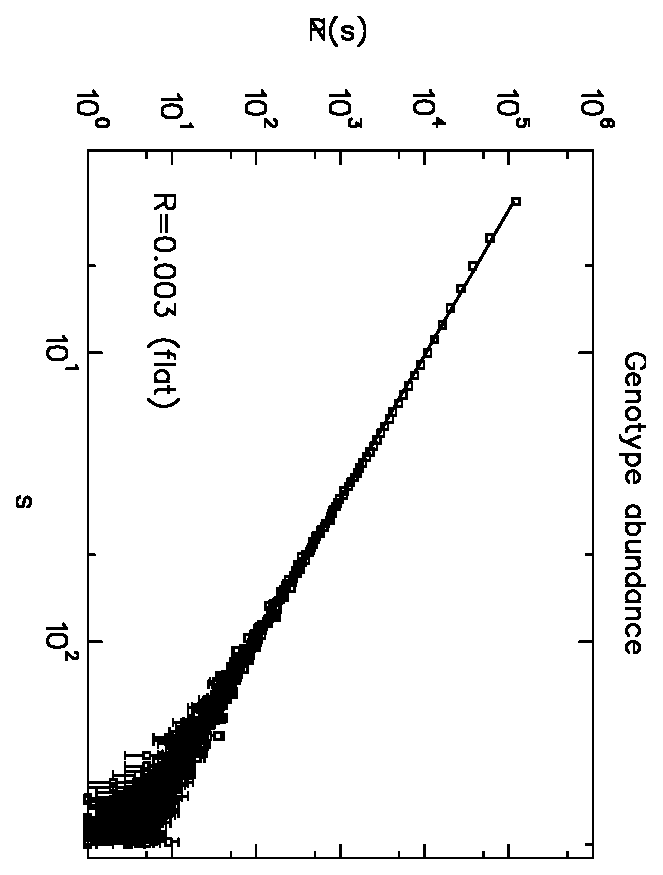
\includegraphics[width=2.25in, angle=90]{fig4.eps}
\caption{Distribution of genotypes sizes $P(s)$ for a landscape devoid
  of the bonuses listed in Tab.~1, at mutation rate $R=0.003$.} \label{fig4}
\end{center}
\end{figure}


Clearly then, even such landscapes (flat with respect to all other
activities except replication) are not neutral. Indeed, it is known
that neutral evolution, where the chance for a genotype to increase or
decrease in number is even, leads to a power law in the abundance
distribution with exponent $D=1.5$ \citep{ABH}.


\begin{figure}[t]
\begin{center}
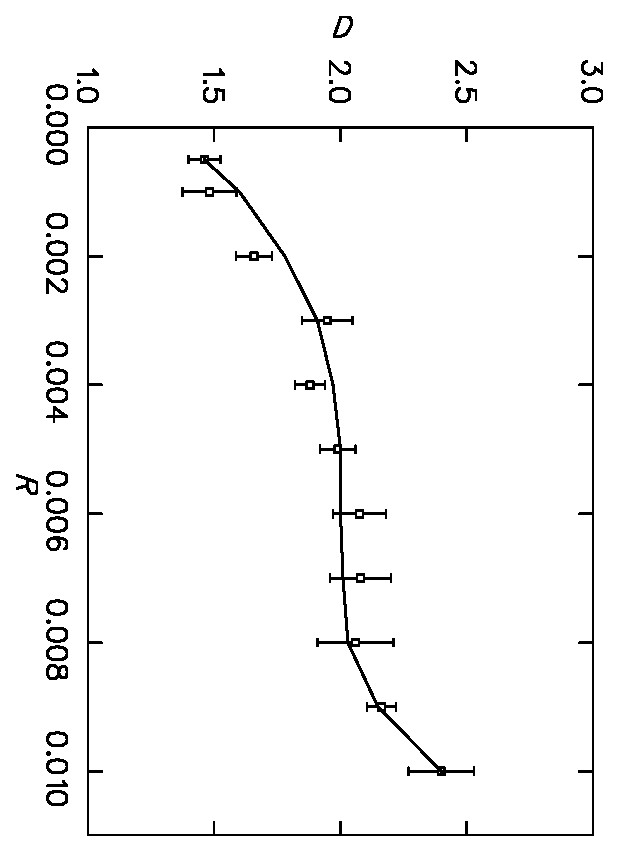
\includegraphics[width=2.2in, angle=90]{fig5.eps}
\vskip 0.25cm
\caption{Fitted exponent of power law for 34 runs at mutation rates
  between $R=0.0005$ and $R=0.01$ copy errors per instruction
  copied. The error bars reflect the standard deviation across the
  sample of runs taken at each mutation rate. The solid line is to
  guide the eye only.
}
\label{fig5}
\end{center}
\end{figure}


In order to test the dependence of the fitted exponent $D(R)$
[Eq.~(\ref{power})] on the mutation rate, we conduct a set of
experiments at varying copy-mutation rates from $0.5\times10^{-3}$ to
$10\times10^{-3}$ and take data for 50,000 updates. Again, a ``best''
genotype is not reached after this time, and we must assume that
avalanches were still occurring at the end of these runs. Furthermore,
in some runs we find that a genotype comes to dominate the population
(usually after most `genes' have been discovered) which carries an
unusual amount of junk instructions. As mentioned earlier, such
species produce a distribution that is exponentially suppressed at
large genotype sizes (data not shown). To avoid contamination from
such species, we stop recording genotypes after a plateau of fitness
was reached, i.e., if the population had discovered most of the
bonuses. Furthermore, in order to minimize finite size effects on the
determination of the critical exponent, we excluded from this fit all
genotype abundances larger than 15, i.e., we only fitted the smallest
abundances. Indeed, at larger mutation rates the higher abundances are
contaminated by a pile-up effect due to the toroidal geometry, while
at lower mutation rates a scale appears to enter which prevents
scale-free behavior. We have not, as yet, been able to determine the
origin of this scale.

In the results reported here, we show the dependence of the fitted
exponent $D$ as a function of the mutation rate $R$ used in the run,
which, however, is a good measure of the mutation probability $P$ only
at small $R$ and if the sequence length is not excessive. As a
consequence, data points at large $R$, as well as runs where an
excessive sequence length developed, carry a systematic error.

\section{Acknowledgements}

This work was supported by NSF grant No.\ PHY-9723972.

\footnotesize
\bibliographystyle{apalike}
\bibliography{example} % replace by the name of your .bib file


\end{document}
